% The main project description file

The story:
\begin{itemize}
    \item Backseat driver: 3 out of 4 Americans are scared of fully autonomous cars [AAA]
    \item In 1900, the driverless elevator was invented - elevators used to have an operator or a 'driver' at all times. It took over fifty years, an elevator operator strike, and a coordinated industry ad campaign for driverless elevators to finally be accepted.
    \item Graceful Handoffs are important - People overtrust..if it works 90\% of time, we think it works 100\% of the time. 
    \item Human in the loop CPS co-design is critical. Generalized to other domains and autonomous systems.
    \item Research has been on modeling human behavior, and interaction.
    \item Specifically want to focus on Trust - hard challenge - trust is a multi-dimensional signal - therefore limit to autonomous vehicles to focus on predictability, and explainability. 
\end{itemize}

\section{Research Description}
%\section{Research Description}
\label{sec:research}

%A subsection labeled "Intellectual Merit" is required in the "Research Description" section of the Project Description.

% Behaviour profile
\subsection{Research Thrust 1: Behavior modeling}
\label{sec:behaviour}

 The ability to (1) detect, (2) assess and (3) manage a person’s emotions has been identified to be the predictor of success in relating to the people around us. By being able to read other’s “emotional cues,” not only we can better understand how they are feeling at a given time, but it also helps us to predict how they will respond in different scenarios. Research suggests that emotions are normally associated with specific events or occurrences (cite), and they can significantly influence our thoughts and behaviors. Additionally, we can use reason to evaluate our emotions, interpret them, and reassess our initial reactions to them. Therefore, by detecting certain events and occurrences, we may be able to assess and predict individual emotional states and use reason to soften their impact or “shift” their meaning. Building on this knowledge, to enhance driver/passenger(s) experience, safety, and trust in the AV, future AVs must be automatically and accurately detect, assess, and manage the passengers behaviors and emotions. Through this approach AVs can better collaborate and communicate with the passengers and develop “human-like” trust with them. 
 
  Within the past two decades, a number of Naturalistic Driving Studies (NDS) aimed at understanding human behaviors in different safety-related conditions, with the specific emphasis towards crash or near-crash incidents. In these studies, cars were equipped with sensors and devices that continuously monitor various aspects of driving behavior such as vehicle acceleration, deceleration, location, and speed, driver-related information such as eye, head and hand movement, and environmental conditions such as traffic and weather conditions (CITE). For instance, in (CITE - European paper) researchers identified that certain driver-personality traits are prone to committing speeding violations; or bad behaviors may cluster together, where drivers who perform one type of risky behavior are more likely to engage in other types of risky behaviors. Although these studies provide significant insights on the driver behavior in different scenarios and contextual settings, they specifically focus only on safety-related behaviors that result in crashes or near-crash incidents; additionally, the first generation of NDS used manual video annotation techniques to identify driver behaviors in specific epochs of driving (CITE), which requires extensive time and manpower to complete. Due to complexities related to human behaviors (i.e., dynamic changes in human behaviors) many of the first generation NDS were limited to short-term monitoring and as a result, lacked in identifying how the driver behaviors may change based on various contextual, environmental, and social settings. With the growing interest in long-term behavioral monitoring and automated monitoring approaches, in more recent NDS studies, researchers are focusing on large-scale computer vision-based and audio processing analyses of human behavior where information can  semi-automatically and/or automatically be extracted from raw video and audio feeds (CITE). For instance, in a recent study from MIT, researchers are using computer vision and voice-processing techniques to monitor drivers body posture, eye movement, and emotions to predict driver's frustration and gaze region that may result in unsafe behaviors while driving semi-automated and fully-automated vehicles (CITE behavioral impact of drivers roles and other MIT work). 
  
    As our cars are moving towards higher levels of autonomy, behavioral and emotional information not only are extremely useful for increasing safety of AVs, they can also be applied towards optimizing control actions of AVs, and most importantly, enhancing the  driving-experience for the driver and/or passenger(s); for instance, by identifying that the driver is feeling “happy,” AVs can optimize their route selection in order to increase the drivers positive emotions, potentially enhancing the driver's mental health. Additionally, by optimizing the decision making of automated systems around the user's specific preferential and comfort profiles, research suggests that the automated system can better gain user trust (cite). Although the more recent NDS are implementing automated monitoring techniques for detecting driver behaviors and emotions, they specifically focus on identifying safety-related behaviors in semi and fully-automated vehicles. As a result, there exists a lack of  understanding on the causation of behaviors as a collective interactions of environmental, emotional, physiological, and social factors (\textit{Gap 1}); and integration of behavioral models into AV safety and control actions(\textit{Gap 2}). Additionally, within the exiting work, limited number of studies have investigated the impacts of social interactions on the driver and passengers behaviors and emotions; by being able to identify the impacts of social interactions on certain behaviors, AVs can better optimize the vehicle's level of autonomy according to the behavioral and emotional states of the driver as well. 

  %current studies also lack real-time data processing.
  
  In this project, we aim to understand how environmental, physiological, and social factors may influence and/or cause certain behaviors and emotions in the driver and passengers. Through instrumenting a number of participant-owned vehicles, we will collect and analyze the impact of different factors on driver/passenger behaviors and emotions. To collect environmental-related information, Automatic Pro (CITE) will be used to monitor the car's speed and location. Automatic Pro will be also used to collect behavioral information such as driver's acceleration and deceleration rates (previous research suggests acceleration/deceleration can be used to identify risky or frustrated drivers (CITE)). Cameras will be used to capture outdoor conditions such as traffic, weather, surrounding cars and pedestrians, signs, infrastructure, etc. as well as indoor conditions such as social interactions, drivers and passenger(s)'s body posture, face, head and hand/arm movement. Ambient-condition sensors will be used to measure thermal settings, indoor and outdoor noise levels, and lighting levels. Audio recorders will be used to capture social interactions as well as any other audio sources (i.e., music, radio, audio books, etc.). Wearables such as Samsung Gear or Fitbit will be used to measure the driver and passengers physiological data (i.e., heart rate and hand/arm movement). Through face recognition software (i.e., OpenSmile, iMotion, and Google API) recorded videos will be processed to create a time-stamped emotional states for the driver and passengers; additionally, audio data will be processed through speech-to-tech and natural language processing techniques to identify and classify various social interactions and audio sources (e.g., music or radio). The audio information as well as physiological information can also be used to identify the driver/passengers emotional states. \ref{fig:sensors} provides an overview of the sensors and data that will be collected from the drivers and passenger(s).   

 To address \textit{Gap 1}, we plan to observe trends in our data that both reveal (1) factors that influence specific human emotions and (2) the downstream consequences of particular emotions on their behaviors. For example, we will aim to understand what environmental (e.g., weather, thermal conditions, lighting, noise) and social factors (e.g., social interaction), physiological factors (e.g.,arm movement) trigger particular emotions. Through this approach, we will also be able to develop a database of  emotions, behaviors and environmental changes. As it may be difficult to often identify triggers to particular emotions (i.e., passenger may appear already experiencing a particular emotion), we plan to evaluate which environmental (indoor and outdoor) and social factors may be used as cues for particular emotions and/or behaviors. For example, as our preliminary data indicates, in rainy conditions, a driver focuses more on his driving, and as a result his acceleration/declaration rates are dropped compared to normal conditions; meanwhile the driver is more likely to not listen to any music. With this information, we will then assess if we can reliably predict particular emotions or behaviors, given specific contextual, environmental or social factor(s); for instance in a rainy condition, the driver will have higher control of the vehicle.The specific research questions that will be addressed through this approach include: 
\begin{enumerate}[itemsep=0pt,parsep=0pt,topsep=4pt,leftmargin=0.4in]
    \item What is the impact of social interaction on driving behavior? 
    \item What is the taxonomy of driving behaviors and emotions based on environmental conditions, social interactions, and physiological changes?
    \item How can driving behavior and emotions be non-intrusively and with least number of sensors be detected?
    \item What are environmental and social factors that impact passenger(s) attention (positively or negatively)? 
    \item Do people have differentiating “trust” profiles according to specific behaviors and contextual conditions?  

\end{enumerate}
 
  By having an understanding about the causation of certain behaviors and emotions (e.g., impact of weather conditions on driving-behavior), behavioral and emotional models can be developed and integrated into AVs systems where they can optimize the control actions as well as feedback/communication strategies based on the driver preferences and behaviors. To achieve this, we propose to develop an Artificial Intelligence (AI) engine that aggregates the information extracted from vision and audio with physiological and environmental information. Through clustering techniques and machine learning algorithms (i.e., CNL and HMM), we will define behavioral models as a function of emotional traits, environmental conditions, social interactions, and physiological measures.%Madhur to improve
  As a result address \textit{Gap 2}, we are specifically interested in formally characterizing emotions and behaviors through a “context-dependence” approach, where spatial and temporal information can be automatically detected, analyzed, and interpreted. Through this approach, behavioral and emotional models can be generated and applied towards:
 \begin{enumerate}[itemsep=0pt,parsep=0pt,topsep=4pt,leftmargin=0.4in]
     \item determining the safety regions according to the reach-ability analysis in Thrust 2 (Section~\ref{sec:reachability}),
     \item as input to the constraints on the control actions to select a trajectory which conforms to the users behavior needs in Thrust 2 (Section~\ref{sec:reachability})
     \item a detection mechanism which triggers when the natural language explanation of the cars actions is generated Thrust 3 (Section~\ref{sec:feedback})
 \end{enumerate}

 
\begin{figure}
    \centering
    \includegraphics[width=0.8\columnwidth]{figures/sensors.png}
    \caption{Overview of instrumentation of vehicles and the collected information from participants}
    \label{fig:sensors}
\end{figure}
 
 


%\begin{center}
    %\begin{tabular}{ | l | l | l |}
    %\hline
    %Type &  Factors & Sensor/Algorithms \\ \hline
    %\multirow{5}{*}{Environmental Sensing} & Speed & Automatic Pro \\
        %& Location & GPS/Automatic Pro \\
       % & indoor and outdoor conditions & cameras \\
      %  & Passengers' identity and count & cameras \\
     %   & Weather Conditions & Camera and weather database\\\hline
    %\multirow{8}{*}{Human Sensing} & Face features & eye tracking, camera, facial recognition \\
       % & Noise levels & noise-level sensors \\
       % & Passenger voice & Voice recorder, Natural Language Processing \\
      %  & Brake and acceleration rate & Automatic Pro \\
     %   & Grip on steering wheel & pressure sensor \\
    %    & Music and other social media use & APIs (e.g., Spotify) \\
   %     & Social interaction & Camera and voice recorder \\ \hline
  %  
 %   \end{tabular}
%\end{center}










% Reach ability + Control Synthesis
\subsection{Research Thrust 2: Reach-ability analysis based safety region estimation}
\label{sec:reachability}
\nicola{This is all you Nicola}
\lu{Lu adds subsection on control synthesis}

% Feedback design 
\subsection{Research Thrust 3: Feedback Design}
\label{sec:feedback}

%\madhur{The primary intellectual merit in this section is the Deep Explanations idea as illustrated in Figure~\ref{fig:deep_exp}. The other part can be on scenario based behavior/trust modeling- but that can be part of the experiment plan too.}

%The purpose of this research thrust is to develop and validate models to quantify trust of a driver in an autonomous vehicles.
The purpose of this research thrust is to develop and validate what feedback should the autonomous vehicle provide to the passengers.

% Trust in self-driving cars is one of the big discussion points in the public debate. 
% Drivers who have always been in complete control of their car are expected to willingly hand over control and blindly trust a technology that could kill them.
% We hypothesize that trust is influenced by three components:
% \begin{enumerate}[itemsep=0pt,parsep=0pt,topsep=4pt,leftmargin=0.4in]
%     \item The person who trusts,
%     \item The system this person is supposed to trust, and
%     \item The driving situation.
% \end{enumerate}

% In addition, the first component (i.e., the person), is characterized by a certain propensity to trust, which is influenced by different factors (e.g., gender, age, opinions, character traits). This is what we want to measure in the proposed research. 

While cars have become significantly more usable — particularly with regard to reliability and safety over the past twenty years — thanks to the introduction of new technologies such as electronic fuel injection, the seat belt, crumple zones, ABS, airbags, electronic stability control and GPS satellite navigation, many of these technologies have succeeded out-of-sight of the humans behind the wheel.
Yet when it comes to newer technologies - like advanced driver assistance systems (ADAS) , we see a much less successful integration of technology, vehicle, and user.
At the broadest level, many of the technologies available in modern cars do not appear to have been developed with a particular user-centred approach. 
They exist because the technology has become available to perform a specific function.

As soon as driving ``feels'' even partly autonomous, people switch off, they become disengaged from the process of driving — and fail to monitor the system. 
A quick YouTube search, reveals many videos where people are aware the systems have limitations, but still push them further than their intended use, operating pilot assist systems on roads or situations when they shouldn't.

We hypothesize, that for autonomous vehicles, trust comes from two factors: \textit{predictabilit}y, and \textit{explainability}.
If a user expects a car to drive in a certain way in a certain situation, and the car conforms to his expectation, the user will tend to trust it more.
Occasionally, when the AV’s action surprise/confuse the user- as long as there is an explanation provided for it, the user can again gauge her level of trust in the system.
Given a proile of the passenger's behavior and emotional needs, from Section~\ref{sec:behaviour} the goal of this researh thrust is to:
\begin{enumerate}[itemsep=0pt,parsep=0pt,topsep=4pt,leftmargin=0.4in]
    \item Develop an automated way to provide explanations for the autonomous vehicle's actions to the passenger - this caters to the \textit{explainability} aspect of a passenger's trust, and
    \item Develop user interfaces which convey the intended actions of the vehicle to the passenger so they can gauge the \textit{predicitability} component of their trust in the autonomous vehicle.
\end{enumerate}

% \subsubsection{Scenario-based trust modeling}
% \label{subsec:trust-modeling}
% \begin{figure}
    \centering
    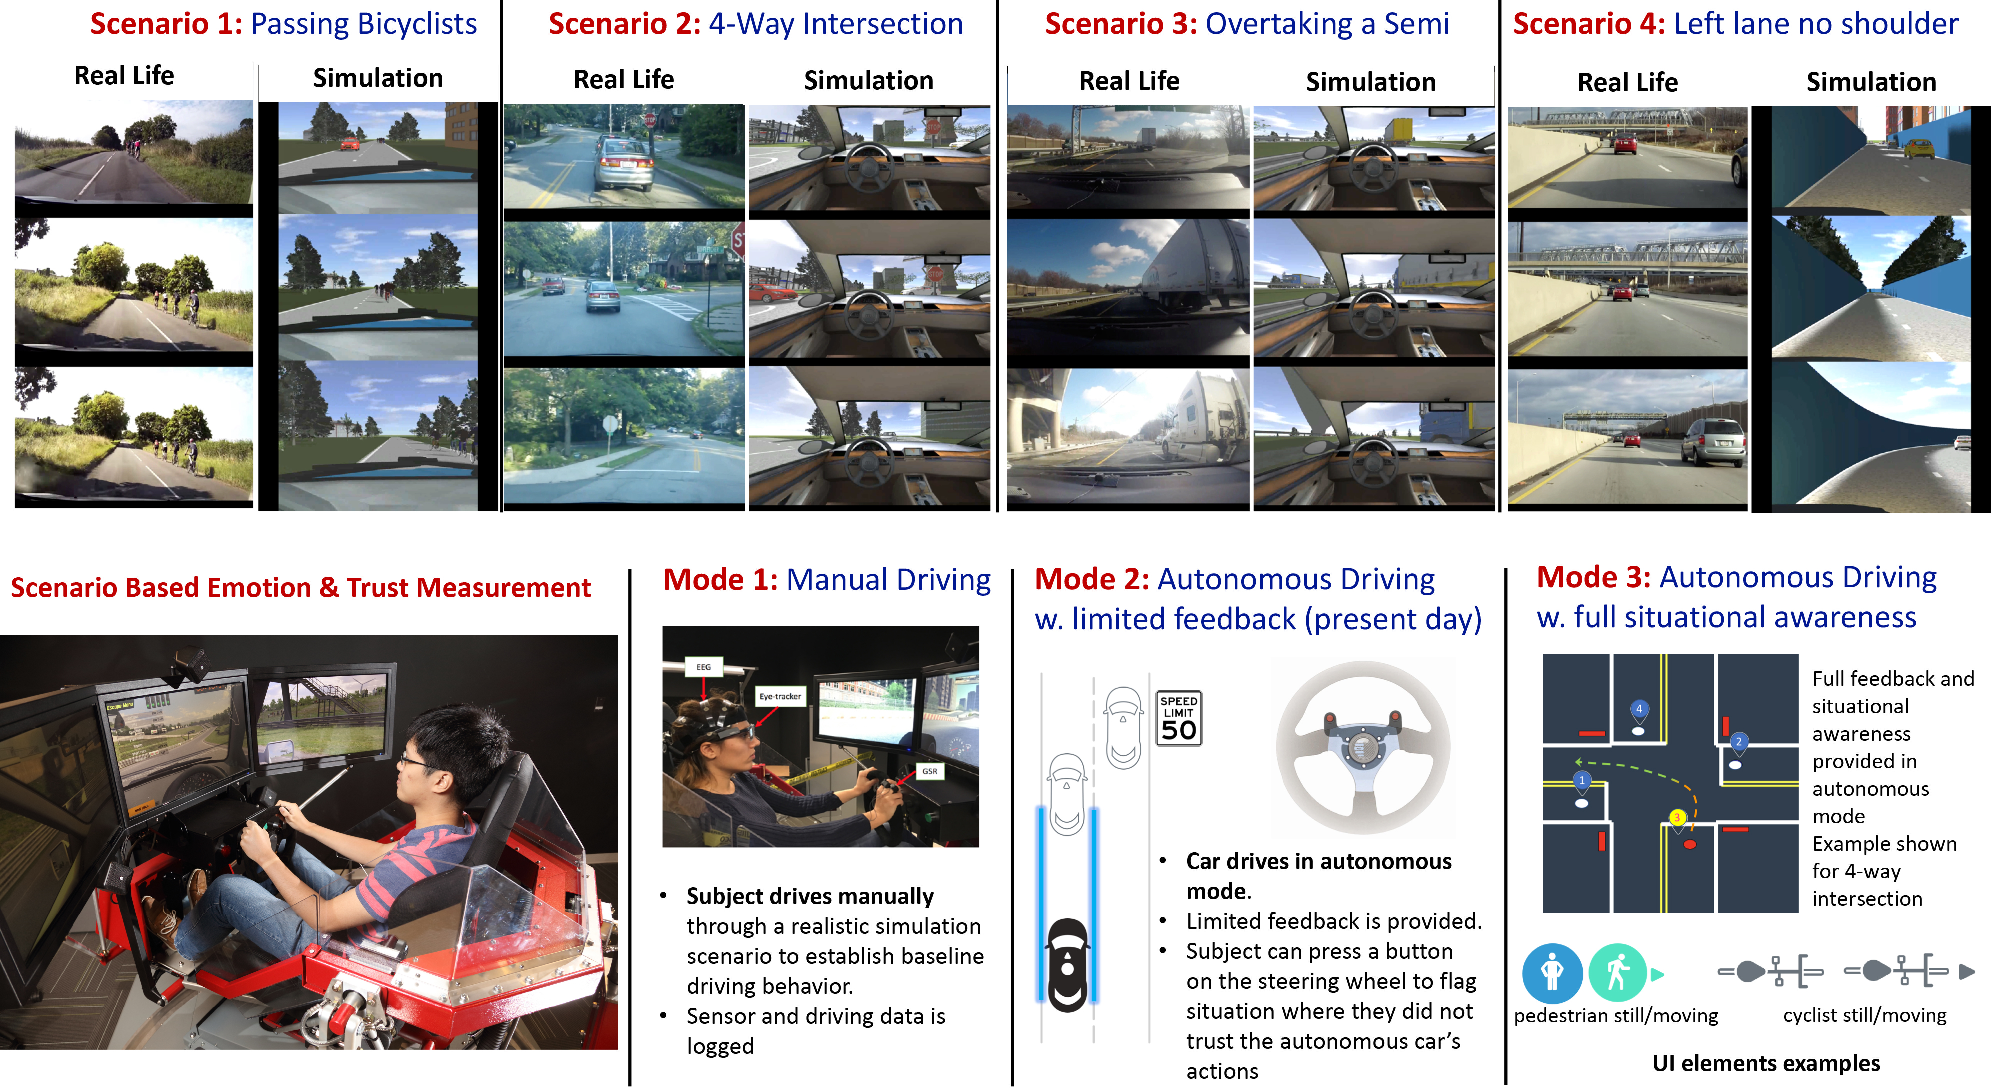
\includegraphics[width=\columnwidth]{figures/scenarios.pdf}
    \caption{Overview of the Scenario Based Emotion and Trust Measurement - We recreate real world traffic situations in simulation using Pre-Scan. During experimentation, we invite human drivers to first manually drive through each scenario (mode 1), followed by an autonomous driving mode where limited feedback and car intentions are provided to the driver, and finally in mode 3, the users experience fully autonomous driving with full feedback and situational awareness provided. We then survey the participants about what feedback enables their trust, which UI elements do they prefer, which mode made them emotionally satisfied.  }
    \label{fig:scenario}
\end{figure}

Behind the wheels of a self-driving car, everyone of a sudden becomes a backseat driver. For thrust 1 on monitoring driver behavior and emotions (Section~\ref{sec:behaviour}, we want to observe and record driver activity in a controlled environment. 
For thrust 3 on feedback design (Section~\ref{sec:feedback}), we want to measure how passengers react to varying degrees of feedback and explanations provided to them by the UI. We setup different traffic scenarios in our full scale driving simulator, to run experiments to gather the data required to build models for human behavior, and test the effectiveness of different kinds of feedback. 
We can simulate multiple scenarios – a four way stop sign, safely passing bicyclists on a narrow road, overtaking a large semi on a freeway, driving too close to a barrier in the absence of a shoulder on the left lane, etc. 

\subsubsection{Participants}
We are proposing to conduct user studies and driving experiments for Thrusts 1, and 3.
The design of a subject study protocol is being undertaken at the time of the witting of the proposal. We are closely working with the Institutional Review Board for Social and Behavioral Sciences at the University of Virginia. The data management plan describes in detail how user data will be recorded, used, distributed, and maintained. A total of at least 100 participants from the University of Virginia will be recruited for participation in this study over 3 years. We we take measures to ensure sufficient diversity within the participation pool. Subjects will be awarded in exchange for participation in accordance with the University of Virginia’s Institutional Review Board practices, and we have requested a budget for the same.


\subsubsection{Setup}
Figure~\ref{fig:scenario} shows the setup of an academic-scale testbed that co-PI Feng's group has partially built and will complete during the proposed effort. The hardware platform is based on the Force Dynamics 401CR driving simulator. This four-axis motion platform can pitch, roll, yaw, and heave, to simulate the experience of being in a vehicle. Thus, we expect to collect data about realistic human response during the driving. The human is interfaced to the hardware platform through PreScan, which is a software tool designed as a development environment for Advanced Driver Assistance Systems (ADAS) and Intelligent Vehicle (IV) systems. PreScan supports virtual sensor technologies such as radar, laser, camera, ultrasonic, GPS and C2C/C2I communications. 
Sensors will be used for both high-level inference of human's intent and preferences and low-level monitoring of human behavioral, mental and physiological states. These sensors include EEG for neural signals, EKG for heart activity, EMG for muscle activity, a camera for head tracking, eye tracking suite and cloud-based speech recognizer.

\subsubsection{Design and procedure}

As shown in Fig.~\ref{fig:scenario}, we have re-created 4 real world driving situations in Pre-Scan - passing bicyclists on a narrow back road, a 4 way intersection, overtaking a semi truck at freeway speeds, and driving on a  freeway in the left lane in the absence of a left shoulder. 
For each of these scenarios, we will conduct the following user experiment:
\begin{enumerate}[itemsep=0pt,parsep=0pt,topsep=4pt,leftmargin=0.4in]
    \item Mode 1 - Manual driving: In this mode, we ask the subject to drive through a given scenario. Each scenario's simulation is a few minutes. While they drive through the scenario, we monitor the person's behavior and emotional cues as well as log their driving behavior. This driving behavior ( steering, brake, acceleration) can be considered as their baseline profile. We also track their gaze, to asses what the driver is paying attention to as they drive. As an example, we will ask the subject to drive through the four way stop sign scenario, where they have to self-asses their right of way as they approach a stop sign. We can then intentionally program one of the agents in the simulation to drive3 out of the order for the right of way and see how the driver adapts. 
    \item Mode 2 - Autonomous driving with limited feedback: Next, we ask the same subject to this time, sit back and relax, as the car drives by itself in the simulator. Everything in the scenario is identical to last time, except that the driving is fully autonomous. We present the driver with a visualization of a virtual dashboard which depicts what the car sees, very similar to what most of the dashboards for semi-autonomous vehicles depict today.  Once again, we monitor the drivers behavioral and emotional cues to interpret their trust in the system. We also give them the option to press a button on the steering wheel, every time they think the car did something that they did not anticipate, or if they mistrusted the car's autonomous driving actions. ``flagging'' these events in a scenario provides us with a basis for designing UI feedback. Continuing with our previous example, a visualization of the four way stop sigh is shown the viewer as feedback, but no indication is given as to if the autonomous car has figured out its right of way, or what is its intended trajectory.
    \item Mode 3 - Autonomous driving with full feedback: Lastly, we have the autonomous car drive through the same scenario one more time, but this time we provide full situational awareness of the scene to the user along with cues about the car's intended actions. In the stop sign example, we project the car's understanding of its right of way, and how that dynamically updates as other vehicles drive through the intersection. We project the cars intended trajectory so the user know that the car will make a left turn and will yield to incoming traffic. More generally, for the parts of the simulation which were flagged by the user, we run the Deep Explanations engine to provide natural language explanations for the car's actions. 
    
\end{enumerate}

Following the experiment, we survey the subjects to understand and gather data on which explanations help increase the trust of the subject, which UI elements work, and to what extent.
Each participant will also be given a questionnaire, adapted from~\cite{merritt2013trust}, to learn about their levels of trust in the autonomous car. 
We will use scales which empirically define the feeling of trust in the autonomous system from~\cite{jian2000foundations} which has been used in many studies about trust~\cite{hoff2015trust}.

\subsubsection{Expected results} 
Upon the completion of data collection, the data will be subjected to a factor analysis to reveal the underlying factor structure of the experimental scale. 
The goal of factor analysis is to condense a larger set of variables to a smaller set of factors, which account for a sizeable proportion of variability within the items. Thus, it is desirable to have a few factors that account for a large portion of the variance. 
A one-way analysis of variance (ANOVA) will also be conducted to examine differences in trust amongst the different driving modes. 
It is anticipated that there will be differences in trust depending on the subject's preferences, driving style, and the autonomous car's behavior. 
More specifically, we anticipate that trust will attenuate with higher levels of feedback. We will create a library of UI elements, a library of simulation scenarios, with detailed statistics about which elements worked and what was the subject's assesment.

In addition, the simulated scenario based experimentation will enable:
\begin{enumerate}[itemsep=0pt,parsep=0pt,topsep=4pt,leftmargin=0.4in]
    \item Creating a library of emotional profiles, and models, of drivers.
    \item Identifying the mapping between the emotional state and the control action of the autonomous car, and vice-versa.
    \item Collect valuable data for training the Deep Explanations networks for natural language feedback.
    \item By deploying the same subject in a real car and monitoring their preferences and driving behavior, we will also validate the realism of the simulation study. 
\end{enumerate}

Although, the simulation setup has a distinct advantage, i.e. repeatability of the same scenario, one of the goals of the proposed work is to develop the proposed models for emotion and driving behavior using data from a real deployment in a car (described later in this section). 




%\madhur{Madhur describes the scenario based experiments with prescan}
% feel free to create another tex input file for this subsection 
%\madhur{I will add some text to this subsection as well.}


\subsubsection{Explainability via Deep-Explanations }
\label{subsec:explainability}

\begin{figure}
    \centering
    \includegraphics[width=\columnwidth]{figures/deep_exp.pdf}
    \caption{Deep-Explanation generation: Each dimension of the scene decomposition is used as an input to caption generation. Representation matching, and seq2seq are then used to generate a likely explanation for the predominant action stream.  }
    \label{fig:deep_exp}
\end{figure}

Automatic image description generation is a challenging problem that has recently received a large amount of interest from the computer vision and natural language processing communities ~\cite{johnson2016densecap, xu2015show, wang2016image, karpathy2015deep,Vinyals2015ShowAT}
Not only must caption generation models be able to solve the computer vision challenges of determining what objects are in an image, but they must also be powerful enough to capture and express their relationships in natural language. 
For this reason, caption generation has long been seen as a difficult problem.
The task of automatic image description involves taking an image, analyzing its visual content, and generating a textual description (typically a sentence) that verbalizes the most salient aspects of the image. 
This requires the joint use of both Computer Vision and Natural Language Processing techniques.
Yet despite the difficult nature of this task, there has been a recent surge of research interest in attacking the image caption generation problem. In particular, deep neural networks have been shown to form new grammatically correct sentences as opposed to the template based models and their limited generalization capability to a novel image.
To capture the correlation between two modalities i.e. visual and natural language we need to map both these to some same space so at learn the relation between them or say we need to learn the multimodal joint model.
Models that uses different deep neural networks like convolutional neural network (CNN), long short term memory(LSTM) networks, recurrent neural network(RNN) to implicitly learn the common embedding. These by far gives the best result on all common datasets of caption generation
Aided by advances in training deep neural networks and the availability of large classification datasets, recent work has significantly improved the quality of caption generation using a combination of convolutional neural networks (convnets) to obtain vector representation of images and recurrent neural networks to decode those representations into natural language sentences.

In the proposed research we extend attention-based image caption generators to work with multidimensional data-sets.
\begin{enumerate}
    \item Instead of generating captions from RGB images alone, we will also generate captions from LIDAR data, depth sensor images, and segmented images. 
    \item The captions themselves, will be enhanced with information about the control decision (steering, acceleration, and braking) made.
    \item We will gather and release a multidimensional caption data-set specifically for autonomous vehicles. 
\end{enumerate}




\subsection{Predictability via UI design}
\label{subsec:uid}
This research analyzes the current scenario and future implications of autonomous driving systems, addressing the creation process of a user interface able to communicate intentions and movements of autonomous vehicle.
The ultimate goal is to increase the confidence felt by the user to this system, encourage inclusion, acceptance and all the benefits it could bring to user mobility, and emotions.
We envision a scenario in which car is not only a tool to get from point A to point B, but a complex device that receives and provides information, is connected to the network, knows traffic situation, programs maintenance, can recognize emotional states, hypothetical distractions and driver physical problems (sleep or tiredness), is able to teach the correct way to drive through feedback and, vice-versa, learning input from the driver.
\begin{wrapfigure}{r}{0.45\textwidth}
  \begin{center}
    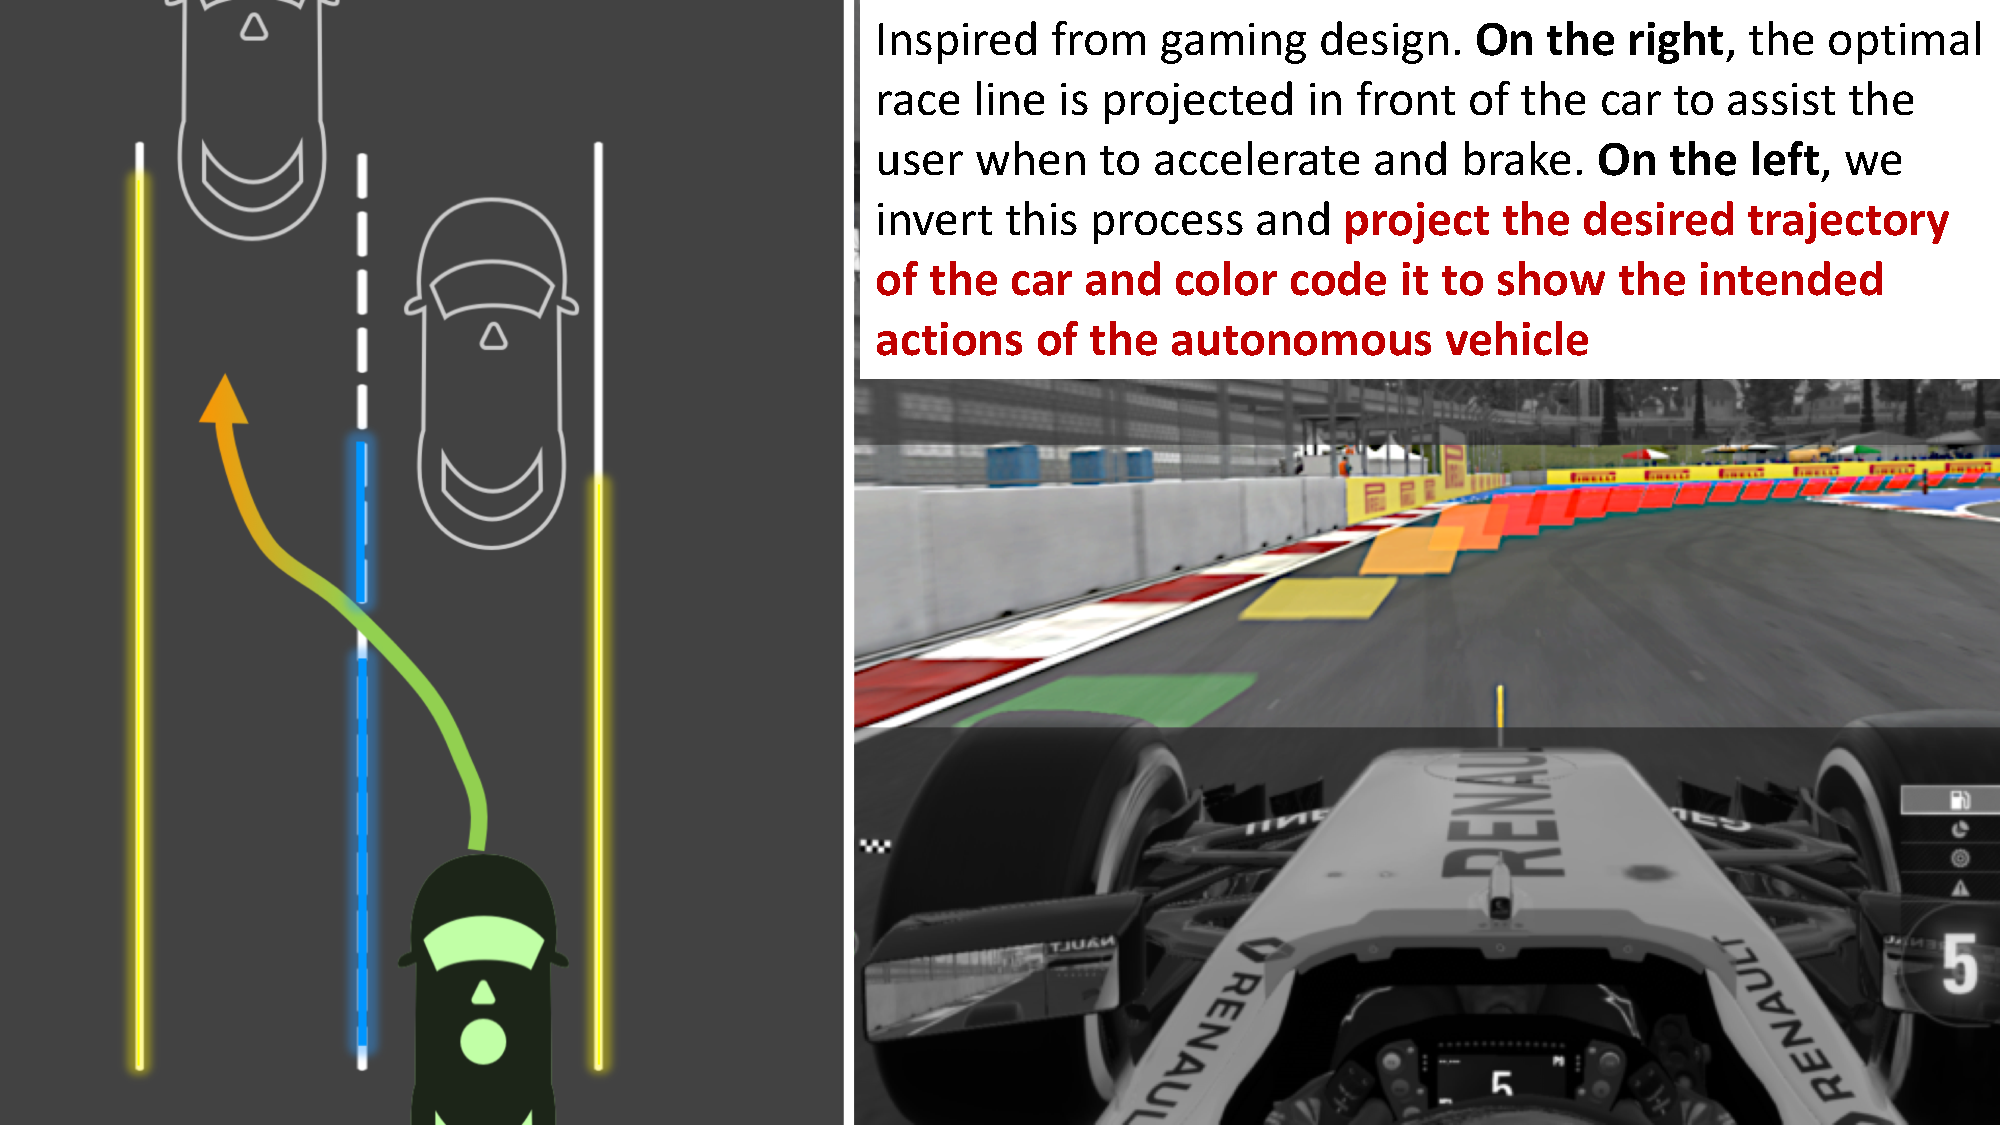
\includegraphics[width=0.43\textwidth]{figures/trajectory_ui.pdf}
  \end{center}
  \caption{Inspired from gaming, projecting the intended trajectory of the car in a color coded manner can realy critical feedback to the user about what actions the car intends to take in any given situation.}
  \label{fig:trajectory}
\end{wrapfigure}
Graphical user interface is an essential tool to create a bridge between the passenger and the autonomous vehicle. 
Present day dashboards/instrument clusters/user interface for semi autonomous vehicles present a high level overview or a wireframe view of what the car sees as its driving. Its typical to highlight lane markings and road signs, and even highlight potential hazards.
However, what is lacking is a design to transparently communicate the intended actions of the vehicle. 
Such transparency is important, because the algorithms by which autonomous cars make decisions are largely invisible to the driver.
If something unexpected occurs, the driver can only speculate what happened. In Section~\ref{subsec:explainability}, we presented an approach to explain the car's actions when driver distress, or a hard braking/steering event occurs. 

In our autonomous vehicle simulator, we will test graphical interfaces design which convey the intention of the autonomous car to the passenger. We are not proposing designing production ready user interfaces for autonomous cars, but a functional study for testing, determining visual variables complexity, information hierarchy and topology, and cognitive load for certain functional UI elements. 
Think of it as a `visual storyboard' of what is happening outside the car. The UI elements will show immediate future movements and choices. ``\textit{Why is the car turning right?}'', ``\textit{Which way is it taking?}'', ``\textit{Can the car detect the cyclist in front of me?}''.
The interface is based on two fundamental principles: simplicity (of use) and anthropomorphism (of language). 
It's not designed for an audience of engineers or designers, it is designed to be as simple as possible, usable and understandable by anyone.

To present a example, we take inspiration from design for motorsport gaming. As shown in Figure~\ref{fig:trajectory}(right), many games project a path in front of the race car to guide the user which is the fastest race line on the track. The color of the race track tells the gamer where to accelerate (green) or slow down (amber). Our idea is to invert this concept for an autonomous car where the UI (Figure~\ref{fig:trajectory}(left)) shows the intended trajectory of the autonomous vehicle and the color of the trajectory coveys if the car will speed up of slow down (brake). We hypothesize that such feedback can help passengers gauge their ``predictability'' metric and hence teir confidence, and trust in the vehicles. 




\subsection{Intellectual Merit}

\begin{itemize}
 \item  Scenario based trust modeling:
    \begin{itemize}
        \item Predictability
        \item Explaniability - Local interpretability. 
        \item Situational awareness and feedback
        \item UI interfaces - A/B testing
    \end{itemize} 
  \item Reachability analysis - linked with predictability and safe handoffs.
  \item Human behavior modeling
  \item Behavior guided autonomy
\end{itemize}

\section{Evaluation/Experimentation Plan}
Testbeds/Experiments:
\begin{itemize}
    \item Reachability experiments with ground robots, F1/10 cars.
    \item UI design kit for Autonomous Vehicles (Matlab, Unity, linked with Pre-Scan)
    \item Driving Simulator: Data to measure trust, predictability, explainability, 
    \item Driver attention and behavior.
    \item Virtual reality testbed ?
    \item What metrics will we use?
\end{itemize}


\section{Project Management and Collaboration Plan}
\begin{itemize}
    \item Perrone Robotics - Letter saying they will allow access to their full scale cars and track.
    \item Toyota Research Institute - Support letter saying they are interested in outcomes of this research and will assist in UI development. 
    \item IRB ?
\end{itemize}
\section{Broader Impacts}

